% Section 1 of the Part B report: replication of Guo & Conitzer (2010).
% Paste into main.tex after the Part A sections.  Figure: results/figures/01_alpha_of_a.png.

\section{Replication of the paper's results}

\subsection{Why replicate}

Both headline numbers of the paper are computational. Theorem~1 ($\alpha\le0.841$ for every
strategy-proof mechanism) is the value of a linear program that the authors solved for one grid
size ($N=50$) without a dual certificate, and Theorem~2 ($0.828\le\alpha(\mathrm{LIP}(2))\le0.829$)
is a numerical sandwich evaluated ``for sufficiently large $N$'' whose $N$ is not reported. Neither
the code nor the intermediate quantities are available. Before extending the model we therefore
re-implemented every computation from the paper's formulas, checked that the stated numbers are
reproduced, recorded the unrounded values and grid sizes the paper omits, and then asked the
two questions the paper leaves open: how the LP bound depends on
the grid, and whether the price parameter $a=2$ is a good choice. All code is in the repository
(\texttt{core/lip.py}, \texttt{core/lp.py}), every number below is produced by
\texttt{notebooks/01\_replication.ipynb} and guarded by automated tests (\texttt{tests/});
software and solvers are listed in Appendix~\ref{app:tools}.

\subsection{Theorem 2: the competitive ratio of LIP(2)}

\emph{Reminder.} Spending $t$ units of currency on an item buys the proportion
$Q(t)=\int_0^t\frac{ds}{as+b}=\frac1a\ln\!\big(1+\tfrac{at}{b}\big)$ of it, with $b=a/(e^a-1)$ so that $Q(1)=1$;
$\alpha(a)=\min_{1\ge x\ge y\ge0}S(x,y)/(x+1-y)$; the paper brackets it on a uniform grid of
step $1/N$ (exact ratio at grid points from above, worst cell corner of each term of $S$ from below,
using the monotonicity of $p_1,p_2$).

\paragraph{What we did.} We implemented exactly this bracket (\texttt{lip.sandwich}) and
verified that a uniform grid reproduces the stated numbers only slowly: the upper bound is
$0.82818$ at $N=50$ and $0.82815$ from $N=100$ on, but the lower bound reaches $0.828$ only for $N\gtrsim 2\cdot10^4$,
i.e. $\sim4\cdot10^8$ cells. We therefore added \emph{adaptive refinement}
(\texttt{lip.sandwich\_adaptive}, \texttt{core/bracket.py}): starting from a $64\times64$ grid, a
cell is split into four only while its lower bound is below the best exact value found so far
minus a tolerance. Since every point of the triangle always lies in some leaf cell, the minimum
of the leaf lower bounds is a valid bound over the whole domain, exactly as in the paper's
argument. With tolerance $10^{-6}$ this needs about $2\cdot10^4$ cells and 30\,ms, and gives
\[
0.8281462\;\le\;\alpha(2)\;\le\;0.8281472,
\]
with the worst profile at $(x,y)\approx(0.4074,0)$: agent~2 wants only item~2, agent~1 mildly
prefers item~2 and, as dictator, buys most of it. This confirms the paper's $[0.828,0.829]$ and
states the same quantity to seven digits. (The paper reports only the rounded bracket and does
not say which $N$ was used, so we cannot tell whether its own computation was less precise or
merely rounded for presentation; the refinement is a computational convenience, not a
correction.) As sanity checks of the dictator rule on which everything else rests, we verified
our implementation against Claim~5 (regime switches at $b/(a+2b)\approx0.119$ and
$(a+b)/(a+2b)\approx0.881$ for $a=2$; the three regimes are the single expression
$t=\operatorname{clip}((x(a+2b)-b)/a,0,1)$), against Lemma~2 (final prices proportional to the
type) and against Example~2 ($0.717$). We also reproduced Figure~1 for $m=3,\ldots,100$ items (Theorem~3; intrinsic value $\theta(a)$
bracketed on a grid of $2000$ points, $a$ scanned on $0.01,\ldots,20$ as in the paper); our
version is Figure~\ref{fig:paper_fig1}.

\begin{figure}[H]\centering
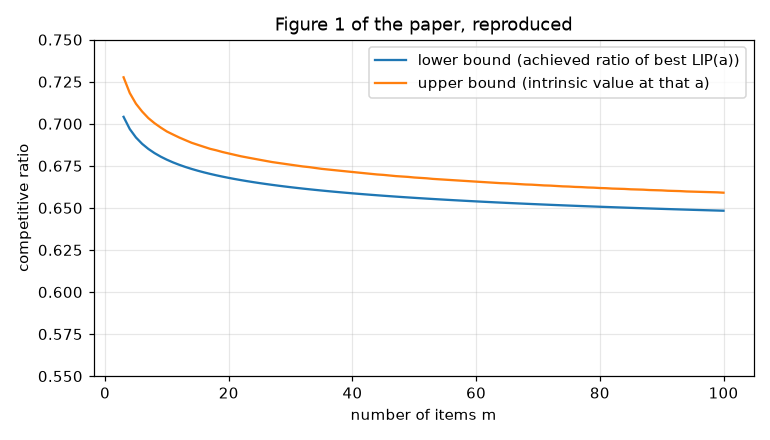
\includegraphics[width=0.8\linewidth]{../results/figures/01_figure1_m_items.png}
\caption{Reproduction of the paper's Figure~1 (Theorem~3): for each $m=3,\ldots,100$ the LIP
parameter $a$ that maximises the lower bound $\frac{a+b}{a+2mb}\,\underline{\theta}(a)$ is chosen
from $\{0.01,\ldots,20\}$; the lower curve is that bound (an achieved competitive ratio), the
upper curve the intrinsic value $\overline{\theta}(a)$ at the same $a$. The best $a$ grows with
$m$ (about $5.0$ at $m=3$, $9.4$ at $m=100$).}
\label{fig:paper_fig1}
\end{figure}

\subsection{Theorem 1: the LP upper bound}

\emph{Reminder.} The argument of Theorem~1 has three steps. (i) Restrict the type space to the
grid $\{j/N\}$: a mechanism only has to serve fewer types, so the best achievable ratio on the
grid is at least the best achievable ratio in general, and any upper bound proved on the grid is
valid in general. (ii) On the grid a mechanism is a finite table: for every report profile
$(j,k)$ the shares $p^1_{jk},p^2_{jk}$ of the two items given to agent~1. (iii) Strategy-proofness
and $\alpha$-competitiveness are linear inequalities in the table entries, so the best mechanism
on the grid is a linear program maximising $\alpha$; the paper solves it for $N=50$.

\paragraph{What we did.} We built the same LP for arbitrary $N$ (\texttt{lp.solve\_sp\_lp}).
The costly part is strategy-proofness: ``no type gains from any misreport against any opponent
report'' is one inequality per triple (true type, misreport, opponent), i.e.\ $(N+1)^3$
inequalities per agent, about $8\cdot10^6$ at $N=200$. We reduce this to $O(N^2)$ by keeping only
the inequalities between \emph{adjacent} types: type $j$ does not want to report $j+1$, and type
$j+1$ does not want to report $j$. This is not an approximation, for the following reason.

Fix the opponent's report $k$. A type $x$ that reports $j'$ obtains
$U(x;j')=x\,p^1_{j'k}+(1-x)\,p^2_{j'k}$, which is \emph{affine in the type} $x$ with slope
$d_{j'}=p^1_{j'k}-p^2_{j'k}$. Two facts follow. First, adding the two adjacent inequalities for
the pair $(j,j+1)$ gives $(x_{j+1}-x_j)(d_{j+1}-d_j)\ge0$: the slopes are non-decreasing in the
report, i.e.\ a higher report yields more of item~1 relative to item~2 (this is implied, not
assumed). Second, with non-decreasing slopes a type that does not gain from moving one step in
some direction does not gain from moving further in that direction either: for $j<j''$,
\[
U(x_j;j'')=U(x_{j+1};j'')+(x_j-x_{j+1})\,d_{j''}
\le U(x_{j+1};j+1)+(x_j-x_{j+1})\,d_{j+1}=U(x_j;j+1)\le U(x_j;j),
\]
using, in order, the (inductively established) truthfulness of $x_{j+1}$ against $j''$, the facts
$x_j-x_{j+1}<0$ and $d_{j''}\ge d_{j+1}$, and the adjacent inequality for $x_j$. The symmetric
chain covers $j''<j$. This is the single-crossing argument familiar from Myerson's lemma:
with utilities linear in a one-dimensional type, strategy-proofness is equivalent to
monotonicity plus local constraints. The same holds in the complementarity model of Part~B,
where utilities remain affine in the type.

We kept the paper's full formulation behind a flag (\texttt{full\_ic=True}) and checked on
grids up to $N=20$ (with and without $\varepsilon$) that both formulations return the same value
to $10^{-7}$; a further test takes the mechanism returned by the reduced LP and verifies
truthfulness against \emph{every} misreport, not only adjacent ones. A second, minor choice is to
impose the agent and item symmetries of the paper's Definition~2 as equalities; by Claim~1 this
does not change the optimum (also verified) and it speeds up the solver several-fold.
With $N=50$ the LP returns $\alpha=0.841225$, the paper's $0.841$.

\paragraph{Beyond the paper: the bound depends on the grid.} Restricting the type space only
removes constraints, so the LP value is a valid upper bound for \emph{every} $N$, and the
smallest value over $N$ is the one to quote. It decreases monotonically:
$0.8429$ ($N=40$), $0.8412$ ($50$), $0.8388$ ($80$), $0.8380$ ($100$), $0.8368$ ($150$),
$0.8363$ ($200$). A least-squares fit $\alpha_N\approx\alpha_\infty+c_1/N+c_2/N^2$ over $N\ge50$
gives $\alpha_\infty\approx0.8345$ (an extrapolation, not a bound). The paper's $0.841$ is the
$N=50$ value and is correct as a bound; finer grids simply give smaller valid bounds, so the gap
between LIP and the best strategy-proof mechanism is less than half of what $0.841$ suggests.

\subsection{Beyond the paper: $a=2$ is not the best LIP mechanism}

The paper evaluates LIP only at $a=2$ and does not motivate the choice. Scanning $a$ with the
certified bracket (step $0.1$ on $[0.5,6]$, then Brent search on $[2.0,2.2]$) gives
\[
a^\star\approx2.1013,\qquad \alpha(a^\star)\approx0.82939\;>\;0.82815=\alpha(2).
\]
Figure~\ref{fig:alpha_a} explains the shape. Two restrictions of the minimisation give
rigorous upper bounds on $\alpha(a)$: along the anti-diagonal $x+y=1$ the ratio is the paper's
own intrinsic value $\theta(a)$ (Claim~8), and along the edge $y=0$ Lemma~2 gives
$Q(t)-Q(1-t)=\ln(\tfrac{x}{1-x})/a$, hence the closed form
\[
\beta(a)=\min_{b/(a+2b)\le x\le(a+b)/(a+2b)}\frac{1+\tfrac x2\big(1+\tfrac1a\ln\tfrac{x}{1-x}\big)}{1+x}.
\]
Numerically $\alpha(a)=\min\{\theta(a),\beta(a)\}$ to $10^{-6}$ on the whole scan: the edge
branch binds for $a<a^\star$, the anti-diagonal for $a>a^\star$, and the optimum is where the
two cross. Steeper prices (larger $a$) make the dictator buy a more balanced bundle, which helps
on the edge and hurts on the anti-diagonal.

\begin{figure}[H]\centering
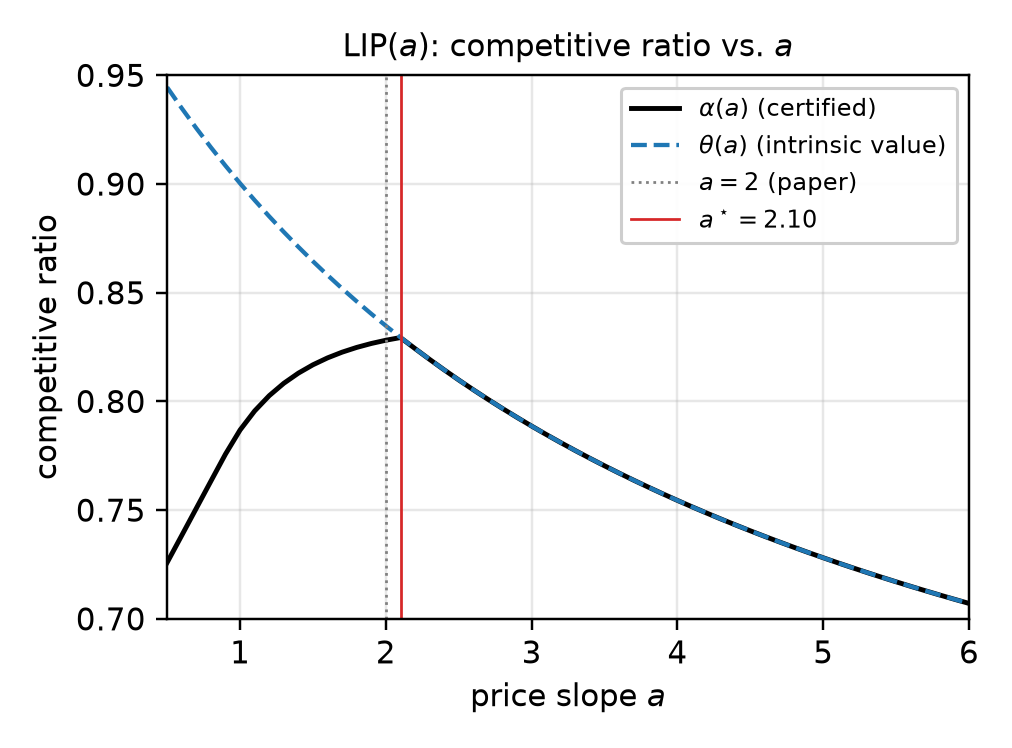
\includegraphics[width=0.95\linewidth]{../results/figures/01_alpha_of_a.png}
\caption{Competitive ratio of LIP($a$) for additive valuations (certified brackets of width
$\le10^{-6}$, black) and the paper's intrinsic value $\theta(a)$ (dashed). The paper's $a=2$ (grey)
and the optimum $a^\star=2.1013$ (red). Right: zoom on the crossing of the two worst-case
branches.}
\label{fig:alpha_a}
\end{figure}

\subsection{Assumptions and caveats}

\begin{itemize}
\item \emph{Rigour of ``certified''.} The brackets are rigorous as mathematical inequalities but
  are evaluated in IEEE double precision, not interval arithmetic; rounding errors are of order
  $10^{-15}$, far below the reported $10^{-6}$ widths.
\item \emph{Grid parity.} LP values for small $N$ depend on whether particular rationals lie on
  the grid; we only draw conclusions from the monotone trend over $N\ge40$.
\item \emph{Extrapolation.} $\alpha_\infty\approx0.8345$ is a curve fit; the only proven
  statement is $\alpha\le0.8363$ ($N=200$).
\item \emph{Two worst-case lines.} That the minimiser of $S/(x+1-y)$ always lies on the edge or
  the anti-diagonal is verified numerically for $a\in[0.5,6]$, not proved; the values
  $\alpha(a)$ themselves do not depend on this.
\item \emph{Replication of Figure~1.} The paper's figure is read off visually; our curves agree
  with it qualitatively (ratios between $0.60$ and $0.73$, decreasing in $m$) but we could not
  compare individual values.
\end{itemize}
